\documentclass[../../main-detail.tex]{subfiles}
\begin{document}
\chapter{表現の構成}\label{chap:practice-foundations}

実践編は，基本体系の表現形成，線形文と照応，語彙分野別の構文，複文と談話の順に構成する．旧版5-2の定義は現行理論に対応させて移植する．口語・文語の文体区分は未決とし，必要な長形を先に与える．

\section{読み方と記法}
\begin{table}[H]
    \centering
    \caption{実践編の記法．}
    \begin{tabular}{lp{0.45\linewidth}l}
    \toprule
    記号 & 意味 & 例 \\
    \midrule
    $t$ & 項位置 & \ko{waka}，\ko{kalam}$^*$ \\
    $R$ & 二項関係位置 & \ko{ja}，\ko{kast} \\
    $R_1$ & 一項述語位置（並置の後項） & \ko{komatci \underline{coto}} \\
    $\_$ & ブランク．省略された項位置 & \ko{\_ kast manomtces} \\
    $x^*$ & 裸の概念語$x$が$F$束縛を受け，発話状況から個体を立てる箇所．$x^{F_i}$のラベルを省いた略記で，形式行では$F_i$を書く & \ko{kalam}$^*$ \sentence{そのりんご} \\
    $t\;r\;t,\;t\;r\;t$ & 形式行の原子文．括弧を付けず，連言はカンマで書く．$[\,\cdot\,]$は関数適用，$(\,\cdot\,)$は順序明記の素の括弧（形式文法章「構文」） & $\ko{waka}\;\ko{ja}\;\ko{hamin}^{F_1}$ \\
    (me) & ソートから補われる関係の転置 & \ko{hamin (me)ke kalam} \\
    \kox{氷} & 未造語．コノメノ語の代わりに日本語を置く & \kox{氷} \ko{tollitam kisa} \\
    \bottomrule
    \end{tabular}
\end{table}
\todo{形式文法に移す}

\paragraph{表層形と形式展開}
例文には，必要に応じて基本体系の式を併記する．\ko{me}や冠詞を明示した形は，同じ文法内で省略を解消した形である．これを別の「保存形」という文体には区分しない．
\begin{exe}
 \ex \ko{waka ja hamin ke kalam}
 \ex \ko{waka ja hamin meke kalam}\hfill 転置を明示
 \ex $\ko{waka}\;\ko{ja}\;\ko{hamin}^{F_1},\;
 \ko{kalam}^{F_2}\;\ko{ke}\;\ko{hamin}^{F_1}$\hfill 形式展開
 \glt 私はりんごを食べる．
\end{exe}
\paragraph{グラフと線形文}
内容の自然な表示は，項を頂点，関係を向き付きの辺とするグラフである（形式文法章「グラフ表示」）．
線形文はグラフを発話順になぞったものであり，矢印と逆向きになぞった辺には\ko{me}が付く．
一筆でなぞれない内容は複数の連鎖に分けてカンマで繋ぐ．このカンマは一つの内容の内部の連言であり，文の切れ目ではない．
\begin{figure}[H]
    \centering
    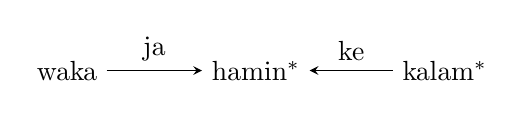
\begin{tikzpicture}[>=stealth, node distance=2.4cm]
        \node (w) {\ko{waka}};
        \node (h) [right of=w] {\ko{hamin}$^*$};
        \node (k) [right of=h] {\ko{kalam}$^*$};
        \draw[->] (w) -- node[above]{\ko{ja}} (h);
        \draw[->] (k) -- node[above]{\ko{ke}} (h);
    \end{tikzpicture}
    \caption{\ko{waka ja hamin ke kalam}のグラフ．\ko{ke}は右から左へなぞるのでこの形では転置が補われる．}
\end{figure}

\section{品詞}\label{sec:practice-pos}

項・述語・冠詞・括弧・心態詞の五つを品詞と呼ぶ．これは語彙についての区分であり，統語的な区分ではない．
\begin{remark}
    統語的に区分する場合，依拠する形式文法のモジュールや規則に沿って区分が複雑化する．項・述語を線形文モジュールの$t$位置・$R$位置に対応させる解説は厳密には正しくない．
\end{remark}
\begin{description}
 \item[項] $A=A_1$．概念と定数を含む．実装辞書では\ko{alkono}に対応する．
 \item[述語] $A_n\ (n\geq2)$．項を関係づける語であり，関数も含む．
 \item[冠詞] $Q^\gamma_{\alpha,\beta}$．項形成と作用域の指定を担う．
 \item[括弧] 表現の範囲や発話の種類を標示する規則上の区分．
 \item[心態詞] 談話モジュールの$N$．返事・挨拶・間投などの慣用表現．
\end{description}
\begin{remark}
    項と述語は$A_n$，つまり$\tArity$で区分されることに注意．$A$は定数と概念を含むが，線形文のパターンは$\arity$によるため，概念（$\arity = 1$）は$t$位置と$R_1$位置の両方に立てるが，定数（$\arity = 0$）は$t$位置にしか立てない．
\end{remark}
\begin{remark}
    括弧は，辞書ではなく規則で導入される各種の表現を寄せ集めた区分である．これらは\ko{[表現1]$\cdots$[表現2]}の形が口語上で共通する．
    \ko{lite}／\ko{liko}は$\tArity=2$の述語なので括弧に含めず，括弧に含める論理演算子は$\lnot$（\ko{meide}$\cdots$\ko{tos}）に限る（2026-09-07暫定）．
    括弧は機能によってさらに区分される（表\ref{tab:practice-brackets}）．形式文法上での対応は，$\{\}$，$()$，$[]$，$\langle\rangle$といった各種の括弧と，論理演算子$\lnot, \land,\cdots$を含む．
\end{remark}
\begin{whynot}
    古い案では型理論・高階論理に基づいた形式理論を構想しており，その際には型が品詞に対応していた（したがって品詞が無限個あった）．
\end{whynot}

% 日本語の名詞・動詞・形容詞に似た区別は，基本的には項のオントロジー上の所属である．特に動詞は述語でないことに注意．

% \ko{ja}「動作主」，\ko{e}「被動作主」，\ko{tov}「所在」，\ko{micto}「所有」，
% \ko{kast}「同一」はいずれも$R_2$である．格助詞・コピュラ・前置詞という名は
% 学習用の小分類であり，形式文法上の別品詞ではない．

% 具体語が分からなければ，\ko{takto}「オブジェクト」，最終的には\ko{alkono}「概念」
% という上位概念で代用できる．裸の上位概念も$F$束縛を受けるため，普通は
% 「文脈上のそのもの」を指す．

\section{形態と構文の接続}\label{sec:practice-morph}
形態規則は，語形の生成と構文への展開を対応させる．個々の派生の定義は，項の形成・述語演算・時制などの使用箇所に置く．
\begin{definition}[形態規則の記述]
一つの形態規則には，次を与える．
\begin{enumerate}
 \item 入力となる語・表現の構文カテゴリと型．
 \item 基本体系の表現への展開と，その出力型．
 \item 語幹・接辞を結合する音韻演算．
\end{enumerate}
展開式がクラス型なら，そのまま個体位置へは置かない．冠詞の適用と名詞化を区別する．複数の派生を合成するときは，内側の出力型と外側の入力型が一致しなければならない．
\end{definition}
\begin{remark}
音韻演算$+$・$\oplus$は，接辞の作用域や意味上の適用順序を決めない．例えば\ko{be+}と複数形成のどちらを先に作用させるかは，括り方の規則で定める必要がある．語形表だけからこの規則は復元できない．
\end{remark}
接辞の音形は，特記しない限り音韻章の母音結合$+$で生成する．人称短縮は子音結合$\oplus$を使う．例えば\ko{hanov}+\ko{oy}＝\ko{hanojoy}，\ko{to}+\ko{oy}＝\ko{tojo}，\ko{komatci}+\ko{ykof}＝\ko{komatcykof}である．
\todo{形態規則を線形文解析の前処理へ接続する．接辞列の構文木・作用域を確定し，展開後の型を検査してから線形文モジュールへ渡す規則を定める．語形だけが同じで展開の異なる候補を，辞書マッチの段階で一つに潰さない．}

\paragraph{ラベル接辞}
添え字$x_n$の語形は，冠詞・括弧・射影・指示詞に共通する．旧版5-2の例外指定を含めて，次のように定める．
\[
 x_n=\begin{cases}
 x+\ko{oy}\ \text{または}\ x+\ko{oi} & n=1,\\
 x+\ko{al} & n=2,\\
 x+(\ko{oi}+n) & n\geq3.
 \end{cases}
\]
$n\geq3$には自然数の乗法形を使う．
\begin{exe}
 \ex \ko{sanoy}, \ko{sanal}, \ko{sanoilu}\hfill 冠詞のラベル1，2，3
 \ex \ko{tojo}, \ko{toal}, \ko{tojolu}\hfill 第1，第2，第3成分への射影
\end{exe}
\begin{remark}
$n=1,2$は形態規則の例外である．\ko{oi}+\ko{y}＝\ko{oy}という音韻上の等式は，乗法形を使う一般則から$n=1$の語形を導いたことにはならない．位取形\ko{y}への切替え自体が追加の指定だからである．旧版の\ko{+oi}という異形態も，この計算だけでは得られない．
\end{remark}
対応が明らかなラベルは省略できる．自然数の語形は\ref{sec:practice-number}を参照．

\section{冠詞と項}\label{sec:practice-terms}
基本体系の項形成を表層形に対応させる．線形文の位置記号$t$と，基本体系の型$V$は区別する．
\begin{definition}[冠詞の二つの構文位置]
冠詞$q$には次の二つの用法がある．
\begin{enumerate}
 \item 一項述語$A:V\to\Omega$に付く$q_i$は，項$A^{q_i}:V$を作る（Plm-at）．語彙上の定数は初めから$V$型であり，この操作を要しない．
 \item 式または項$u$を囲む$q_I$は，$\{u\;q_I\}$を作る（Plm-pt）．内部の$q_i$とラベルで対応し，$u$の入力型と結果型は冠詞署名で定まる．
\end{enumerate}
例えば，$\{\phi\;\forall_I\}:\Omega$に対し，$\{\phi\;L_1\}:V\to\Omega$である．後者は条件を満たす個体のクラスであって，個体項ではない．
\end{definition}
\begin{remark}
冠詞を項に付ける操作と，その作用域を閉じる操作は別である．冠詞の基本形・括弧端形はこの二位置に対応する．一文全体を作用域とする括弧の省略も，この対応を消さない．
\end{remark}

\subsection{冠詞の基本形}
冠詞の語形は「冠詞と括弧の語形」の節の表にまとめた．ここでは項に付く基本形の使い方だけを見る．
量化系は後置，集合化系は前置が無標で，冠詞全体に一つの位置規則はない．
\ko{+ta}を付けた\ko{santa}，\ko{leta}などは主要部を省いた形で，\ko{santa}「すべて」，\ko{leta}「そのようなもの」のように使う．
\begin{exe}
    \ex \ko{coto san wal nanoy to kalam kon}\hfill \sentence{誰もが何かりんごを愛する}
    \ex \ko{ena coto}（＝\ko{eto}）\hfill \sentence{誰}
    \ex \ko{les} $\phi(\ko{le coto})$ \ko{fol}\hfill \sentence{$\phi$である人（たち）}．形式は$\{\phi(\ko{coto}^{L_1})\; L_1\}$
    \ex \ko{kalam anic}\hfill \sentence{何でもよいあるりんご}
\end{exe}
\ko{anic}は「彼は医者を探している」の不特定読みに使う．特定の医者なら裸語でよい．

\subsection{クラスと集合個体}
\begin{itemize}
 \item \ko{coto}の項位置での出現は，$\ko{coto}^{F_i}:V$の略記である．人の外延全体ではなく，文脈から選ぶ人を指す．
 \item \ko{cotoim}は，名詞化子$\setop{\ko{coto}}:V$である．定義される場合に限り，人の外延を集合個体として指す．
 \item \ko{komatcykof}は小町の単元集合を指す．\ko{+ykof}の入力は個体，\ko{+im}の入力はクラスである（\ref{sec:practice-logic}）．
\end{itemize}
\begin{remark}
名詞化子は部分関数である．\ko{*fonneim}のような未定義の名詞化を含む原子文は偽になる（形式文法章「名詞化子と部分性」）．$L$でクラスを作れたことは，そのクラスを名詞化できることを意味しない．
\end{remark}

\subsection{外複数}\label{subsec:practice-outerplural}
個体$a$の外複数は，$a$を要素に持つ集合のクラスである．
\[
 \ko{$a$+na}=\ko{les $a$ litoi leta fol}.
\]
概念語$A$に付ける場合は，先に$A^{F_i}$を選び，この個体を$a$に代入する．内複数と違い，他の構成員が$A$に属することは要求しない．例えば\ko{cotona}は，選ばれた人を含む集合を表す．
\begin{remark}
集合のクラスを作る操作と，そこから特定の集合を選ぶ$F$は区別する．「私たち」のような項で用いる場合は，外複数のクラスから文脈に適した集合を選ぶ．内複数は\ref{par:counted-plural}を参照．
\end{remark}

\section{冠詞と括弧の語形}\label{sec:practice-forms}
冠詞と括弧の語形をまとめる．使い方は「冠詞と項」「括弧と作用域」「文の種類と定型」の各節に置く．
冠詞には項に付く\textbf{基本形}と，作用域括弧の端に置く\textbf{括弧端形}がある．「位置」は項に付くときの無標の側で，括弧では前後どちらの端に置いてもよい．
\begin{table}[H]
    \centering
    \caption{冠詞の語形．}\label{tab:practice-articles}
    \begin{tabular}{lllll}
        \toprule
        演算子 & 基本形（項） & 括弧端形（括弧） & 位置 & 意味 \\
        \midrule
        $F$ & （省略）/\ko{fe} & \ko{fes} & 前置 & 外界照応・談話指示子導入 \\
        $\forall$ & \ko{san}/\ko{santa} & \ko{sas}/\ko{sasta} & 後置 & 全称 \\
        $\exists$ & \ko{kon}/\ko{konta} & \ko{kos}/\ko{kosta} & 後置 & 存在 \\
        $\mathrm{Most}$ & \ko{fante} & \ko{fans} & 後置 & ほとんどの \\
        $\mathrm{Many}$ & \ko{mefante} & \ko{mefans} & 後置 & 少なくない \\
        $\exists$の糖衣 & \ko{anic} & \ko{aninok} & 後置 & 不特定の \\
        $L$ & \ko{le}/\ko{leta} & \ko{les}/\ko{lesta} & 前置 & 条件を満たすクラス \\
        $\mathrm{Lf}$ & \ko{laf}/\ko{lafta} & \ko{lafis} & 前置 & ラムダ抽象 \\
        $E$ & \ko{ena} & \ko{ha} $\cdots$ \ko{tos}（暫定） & 前置 & 疑問「どの」・選択肢化 \\
        $K$ & \ko{sun} & \ko{sus} & 後置 & 命題化・様相 \\
        $[K]$／$\langle K\rangle$ & \ko{sunsan}／\ko{sunkon} & \ko{sunsas}／\ko{sunkos} & 後置 & 必然／可能 \\
        \bottomrule
    \end{tabular}
\end{table}
\ko{+ta}を付けた\ko{santa}，\ko{leta}などは主要部を省いた形である．量化系（\ko{san}, \ko{kon}, \ko{fante}, \ko{anic}, \ko{sun}）は後置，集合化系（\ko{le}, \ko{laf}, \ko{fe}）は前置が無標で，冠詞全体に一つの位置規則はない．

括弧は，辞書ではなく規則で導入される表現をまとめた区分である（「品詞」の節）．
\begin{table}[H]
    \centering
    \caption{括弧の語形．$q$は基本形，$q'$は括弧端形．}\label{tab:practice-brackets}
    \begin{tabular}{llp{0.36\linewidth}l}
        \toprule
        口語 & 形式 & 用途 & 説明する節 \\
        \midrule
        \ko{cu} $\phi$ \ko{nais} & $(\phi)$ & 素の括弧．演算の順序を明示するだけ & 括弧と作用域 \\
        \ko{cu} $\phi$ $q$ & $\{\phi\; F\}^{q}$ & 中の裸項を$F$でまとめ，その項に$q$を後置 & 括弧と作用域 \\
        \ko{fol} $\phi$ $q'$／$q'$ $\phi$ \ko{fol} & $\{\phi\; q_I\}$ & $q$が中の接辞項を束縛する作用域括弧 & 括弧と作用域 \\
        \ko{meide} $\phi$ \ko{tos} & $\lnot\phi$ & 文否定 & 括弧と作用域 \\
        \ko{ha} $\phi$ \ko{tos}／\ko{no} & $\{\phi\; E_I\}$ & 選択肢・疑問 & 文の種類と定型 \\
        \ko{hato} $\phi$ \ko{tos} & $\{(\phi\lor\lnot\phi)\; E\}$ & 二択疑問 & 文の種類と定型 \\
        \ko{min} $\phi$ \ko{tos} & $\{\phi\; M\}$ & 表現の引用 & 括弧と作用域 \\
        \ko{minac} $\phi$ \ko{tos} & （記号列） & 文字列の引用 & 括弧と作用域 \\
        \ko{floi} $x_1 \cdots x_n$ \ko{tos} & $\langle x_1,\ldots,x_n\rangle$ & 順序組 & 論理と集合 \\
        \ko{fonoi} $x_1 \cdots x_n$ \ko{tos} & $\{x_1,\ldots,x_n\}$ & 集合の列挙 & 論理と集合 \\
        \bottomrule
    \end{tabular}
\end{table}

\section{括弧と作用域}

\subsection{量化}\label{subsec:practice-quant}
冠詞の二つの構文位置は\ref{sec:practice-terms}で定義した．ここでは括弧端形によって作用域を明示する．
\begin{remark}
5-2の接続形は，現行では括弧端形へ移している．\ko{fol coto san}の\ko{san}は項に付く基本形であり，これだけでは全称量化の括弧端にならない．括弧を閉じる位置では\ko{sas}を使う．
\end{remark}

\paragraph{3種類の括弧}
括弧の語形と形式対応は「冠詞と括弧の語形」の節の表にある．$q$は基本形，$q'$は括弧端形である．\ko{cu} $\cdots$ \ko{nais}は$(1+2)+3$のような
順序明記のための括弧であり，$\{\ \}$とは別物である．\ko{cu} $\phi$ $q$は
\ko{cu} $\phi$ \ko{nais} $q$の短縮とみなせる．

\ko{fol}は作用域括弧の中立標識である．冠詞は括弧のどちらの端に置いてもよく，
\ko{fol}が空いた側を埋める．
\begin{exe}
    \ex \ko{fol} $\phi$ \ko{sasoy}\hfill 作用域を最後に閉じる（無標）
    \ex \ko{sasoy} $\phi$ \ko{fol}\hfill 作用域を先に宣言する
\end{exe}
量化系（\ko{san}, \ko{kon}, \ko{fante}, \ko{anic}, \ko{sun}）は後置，
集合化系（\ko{le}, \ko{laf}, \ko{fe}）は前置が無標で，項に付くときの側と一致する．
5-2で基本形と接続形の対立が担っていた「作用域の開始を先に言うか」の区別は，
語形の対立ではなく冠詞を括弧のどちらの端に置くかの対立になる．

\paragraph{スコープの言い分け}
文の一番外側の括弧は省略できるので，内側を一つ括るだけで多義が解ける．括弧で明示した側が
内側（狭い作用域）になり，もう一方は省略された最外括弧に束縛される．
\begin{exe}
    \ex \ko{coto san wal nanoy to coto kon}\hfill 無標（表層順）
    \ex \ko{fol coto sanoy wal nanoy to coto konal kosal}\hfill $\forall > \exists$
    \ex \ko{fol coto sanoy wal nanoy to coto konal sasoy}\hfill $\exists > \forall$
\end{exe}
明示がなければ接辞項は文末で左から順に閉じる（左にあるものほど広い）ものとする（5-2は基本形の作用域を単に曖昧としていた）．
副産物として，否定を越える量化のために5-2が用意していた脱出接辞\ko{mo}$+Q$
（\ko{mosan}）は不要になる：\ko{meide} $\cdots$ \ko{tos}の外側に\ko{fol} $\cdots$ \ko{sas}
を置けばよい．

\paragraph{$F$の一括束縛}
5-2の\ko{kostafe}（＝\ko{kosta felilee}）は$\{\phi\; F\exists\}$，
すなわち$\{[\{\phi\; F\}^{\exists}\; A]\;\exists\}$の略記であった．現行文法では$A$（\ko{alkono}）と
最外括弧を省略できるので，\ko{cu} $\phi$ \ko{kon}を単独で文として使えばこれになる．
\begin{exe}
    \ex \ko{cu fylam ansa kalam kon}\hfill 赤いりんごがある
\end{exe}
\ko{felilee}系の語彙を別に立てる必要はない．\ko{kostafe}は歴史的な語形として残す．

\paragraph{命題化と様相（\ko{sun}）}
$K$は文から，それが真になる世界のクラスを作る演算子である（形式文法「フレームと命題化演算子」）。
口語形\ko{sun}は音列\ko{su}「書く・文字・世界」と語彙\ko{suis}「世界」に由来し，
\ko{san}・\ko{kon}と同じ軽音節CVNの語形を持つ．$[K]$（必然$\Box$）と$\langle K\rangle$（可能$\Diamond$）は
\ko{sun}に量化冠詞を後続させた合成形とする（語形\ko{sunsan}/\ko{sunkon}は暫定）．
\begin{table}[H]
    \centering
    \begin{tabular}{llll}
        \toprule
        演算子 & 基本形 & 括弧端形 & 意味 \\
        \midrule
        $K$ & \ko{sun} & \ko{sus} & $\phi$が成り立つ世界たち＝命題 \\
        $[K]$ & \ko{sunsan} & \ko{sunsas} & 必然（全ての世界で） \\
        $\langle K\rangle$ & \ko{sunkon} & \ko{sunkos} & 可能（ある世界で） \\
        \bottomrule
    \end{tabular}
\end{table}
\begin{exe}
    \ex \ko{fol kaja hamin ke kalam sunkos}\hfill 彼がりんごを食べることはありうる
    \ex \ko{fol kaja hamin ke kalam sunsas}\hfill 彼は必ずりんごを食べる
    \ex \ko{walka loyst to fol coto tov kuistent sus}\hfill 私はその人が学校にいることを知っている
\end{exe}
最後の例は5-2の\ko{walka loyst to min coto tov kuistent}に対応する．\ko{min} $\cdots$ \ko{tos}は
$\{\cdots M\}$，すなわち表現をオブジェクトとして扱う演算子であり，世界の集合としての命題を
作る\ko{sun}とは別物である（\ko{minac} $\cdots$ \ko{tos}は記号列で，これも別）．
\ko{loyst}「知る」がどちらを取るかは未決である．

\ko{fol}は音列\ko{folka}「カゴ・体系・枠組み」に由来する新造語である．音列\ko{flo}「一列の」・括弧\ko{floi} $\cdots$ \ko{tos}（順序対）と音が近く，口頭での混同可能性は未検証である．

\subsection{否定}
一語の述語$R$の否定は\ko{be+R}，命題$\phi$全体の否定は
\ko{meide} $\phi$ \ko{tos}で表す．前者は原子的否定，後者はスコープを持つ文否定であり，
量化子を含むと一般に同義でない．

\section{述語の派生}\label{sec:practice-derivation}
\begin{definition}[存在量化による項の取り出し]
$n$項述語$R\in R_n$の第$i$項を残し，他の項を存在量化する．$i=1,2,3$の語形を，それぞれ\ko{$R$+esk}，\ko{$R$+ene}，\ko{$R$+kisk}とする（$i\leq n$）．例えば二項関係では，
\begin{align*}
 \ko{$R$+esk}&=\{\{V^{L_1}\;R\;V^{\exists_2}\;\exists_2\}\;L_1\},\\
 \ko{$R$+ene}&=\{\{V^{\exists_1}\;R\;V^{L_2}\;\exists_1\}\;L_2\}.
\end{align*}
一般の$n$では，残す項に$L_i$を付け，それ以外の$n-1$項をそれぞれ$\exists_j$で閉じた式を$L_i$で抽象する．出力型は$V\to\Omega$である．旧版5-2は$i\geq4$を\ko{$R$+(kn$\oplus i$)}と書く．これも同じ項射影であり，音形の生成には音韻章の演算を用いる．
\end{definition}
\begin{exe}
 \ex \ko{komatci miblalisesk}\hfill 小町は誰かの子である．
 \ex \ko{komatci miblalisene}\hfill 小町には子がいる．
\end{exe}
\begin{remark}
\ko{+esk}は単に第1項の辞書上の定義域を返す演算ではない．実際に関係を満たす相手の存在を要求する．また，残す項以外の値を指定する片側固定とは異なる．
\end{remark}
\paragraph{片側固定}
現行の暫定規約では，\ko{+oy}は第1項，\ko{+al}は第2項を固定する．固定する個体を$a$とすれば，
\[
 \ko{les $a$ $R$ leta fol},\qquad
 \ko{les leta $R$ $a$ fol}
\]
がそれぞれの長形である．
\memo{旧版5-2「基本的な記法」は，固定引数と抽象する引数の説明が揺れており，後半の$y\;R+\mathrm{oy}$・$x\;R+\mathrm{al}$は現行の番号付けと逆になる．上では現行の暫定裁定を維持した．接辞付き語の前後どちらに固定引数を置くかも含め，語形と長形を一対一に対応させる必要がある．}
\paragraph{述語否定}
\ko{be+$R$}は，$R$の各引数を保ったまま原子式を否定する．文全体の否定は\ko{meide} $\phi$ \ko{tos}であり，量化作用域を含む場合には区別する．

\section{論理と集合}\label{sec:practice-logic}
論理演算・集合演算と，それに項を渡すための操作をまとめる．これらは形式文法章の語彙定義に由来し，オントロジー上は\ko{loka}（\ko{mintos}・\ko{fonne}）とその関係である．
項の取り出しと片側固定は\ref{sec:practice-derivation}で定義した．ここでは論理結合と集合の構成を扱う．

\paragraph{論理演算}
命題を結ぶ演算と，一項述語を項ごとに結ぶ演算（$f\mathbin{@'}g = \lambda x,\,f(x)\mathbin{@}g(x)$）が対になっている．
\begin{center}
\begin{tabular}{lllllll}
    \toprule
    & 論理和 & 論理積 & 含意 & 非含意 & 同値 & 排他的論理和 \\
    \midrule
    論理演算 & \ko{liko} & \ko{lite} & \ko{lista} & \ko{belista} & \ko{kalista} & \ko{delista} \\
    述語演算 & \ko{miko} & \ko{mite} & \ko{lissa} & \ko{belissa} & \ko{kalissa} & \ko{delissa} \\
    \bottomrule
\end{tabular}
\end{center}
恒真は\ko{konston}，恒偽は\ko{bailek}，命題そのものは\ko{mintos}である．命題の並置は\ko{lite}の省略として読む（「文をつなぐ」の節）．述語演算の\ko{miko}・\ko{mite}は，集合とみたときの$\cup$・$\cap$である．
\memo{現版では厳密に1階しか許さないので，述語演算→集合演算にする．述語演算はwhynotに入れる←いややっぱり述語演算はほしい．集合演算と分けて3段にする}

\paragraph{順序対と射影}
順序対$\langle x,y\rangle$は\ko{$x$ te $y$}と書く．\ko{te}は二項のコンストラクタであり（形式文法章の語彙定義．辞書v5でも二項関数，id 1046），三つ以上の組は入れ子\ko{cu $x$ te $y$ nais te $z$}か次の括弧形で書く（2026-09-03，暫定）．括弧形\ko{floi} $x_1\;\cdots\;x_n$ \ko{tos}も
同じ組を作り，こちらは要素数を口頭で確定できる．第$n$成分への射影は，ラベル接辞
（\ref{sec:practice-morph}）を\ko{to}に付けて作る．
\begin{exe}
    \ex \ko{tojo}, \ko{toal}, \ko{tojolu}\hfill 第1・第2・第3成分
\end{exe}
5-2は第1・第2成分を\ko{toi}・\ko{tal}と書いていたが，これは現行のラベル系列から導けない語形である．

\paragraph{集合の構成}
要素を並べて集合を作る括弧は\ko{fonoi} $x_1\;\cdots\;x_n$ \ko{tos}である．
所属$\in$は\ko{litoi}，包含$\subseteq$は\ko{skon}，等号$=$は\ko{kast}，
和集合$\cup$は\ko{miko}，共通部分$\cap$は\ko{mite}である．

個体$x$からその単元集合$\{x\}$を作る接辞は\ko{+ykof}である．音列\ko{ko}「1・粒・孤独な」と
\ko{fon}「小さめの袋・閉曲面」の合成\ko{kof}に接続用の\ko{y}を前置したもので，材料は\ko{kwilfon}「空集合」と同じ系列にある．
\begin{exe}
    \ex \ko{komatcykof}\hfill $\{$小町$\}$
    \ex \ko{komatci litoi komatcykof}\hfill 小町は$\{$小町$\}$の要素である
\end{exe}
\ko{+ykof}は原始的な操作ではなく，\ko{les le alkono kast} $x$ \ko{fol}に\ko{+im}を付けた形の
略記である（形式文法章の語彙の定義とその直後のremark）．個体の単元集合は常に個体なので，
名詞化子の部分性はここでは問題にならない．\ko{fonoi} $x$ \ko{tos}でも単元集合は作れるが，\ko{+ykof}は括弧を開かずに項を集合位置へ上げられる点で短い．

5-2は$\{x,y\}$を\ko{$x$ mi $y$}（\ko{miko}の短縮）と書き，その根拠に$x$と$\{x\}$の同一視を
置いていた．現行文法はこの同一視を採らない（「コピュラ文」の小節）ので，
\ko{miko}の両項は初めから集合でなければならない．\ko{+ykof}を明示的に置けば5-2の短縮は
そのまま復元でき，$\{x,y\}$は次の2通りで書ける．
\begin{exe}
    \ex \ko{fonoi $x$ $y$ tos}\hfill 要素を並べる括弧形
    \ex \ko{$x$ykof miko $y$ykof}\hfill 単元集合の和
\end{exe}
つまり5-2の\ko{mi}が担っていた仕事は，同一視ではなく\ko{+ykof}という形態素として書く．
\ko{mi}自体を集合形成に使わない理由は「文をつなぐ」の節を参照．

クラスを\ko{litoi}の右項や\ko{te}の項に置くには名詞化\ko{+im}が要る．裸のクラスは項位置に立てない．
\ko{+im}がクラスを個体へ落とすのに対し，\ko{+ykof}は個体を集合個体へ上げる．

\paragraph{直積・直和・指数}
集合$\alpha,\beta$に対して，$\alpha\times\beta$は\ko{$\alpha$ stolite $\beta$}，$\alpha+\beta$は\ko{$\alpha$ stoliko $\beta$}，$\beta^\alpha$は\ko{$\alpha$ stolista $\beta$}である．述語演算の語幹に\ko{sto}を前置した系列で，型（値空間）の構成に使う．


\end{document}
